\documentclass[tikz]{standalone}
\begin{document}
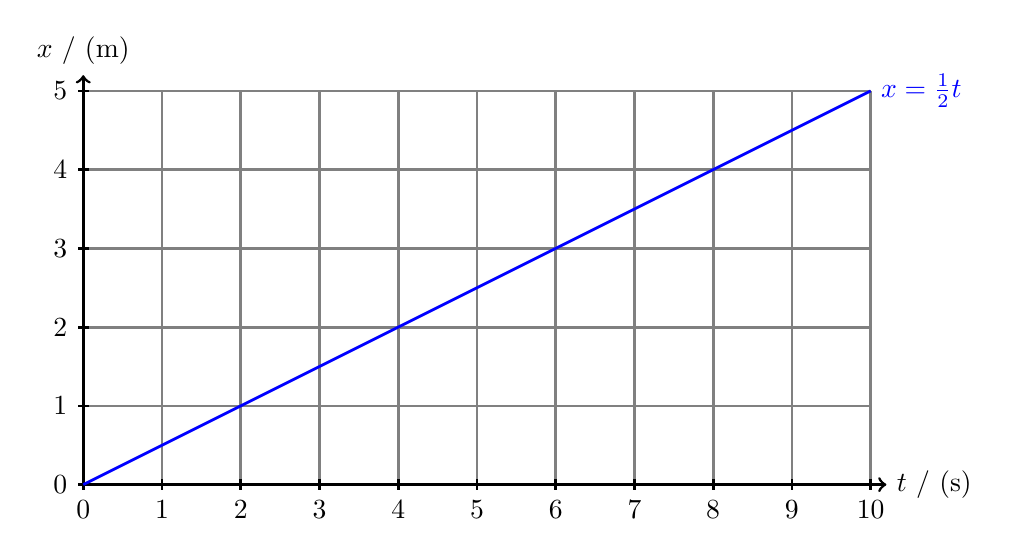
\begin{tikzpicture}[scale = 1, line width = 1pt, domain = 0:10]
\draw[color = gray] (0, 0) grid (10, 5);
\draw[->] (0, 0) -- (10.2, 0) node[right] {$t$ / (s)};
\draw[->] (0, 0) -- (0, 5.2) node[above] {$x$ / (m)};
\foreach \x in {0,...,10} \draw (\x, 2pt) -- (\x, -2pt) node[anchor = north] {\x};
\foreach \y in {0,...,5} \draw (2pt, \y) -- (-2pt, \y) node[anchor = east] {\y};
\draw[color = blue] plot (\x, 0.5 * \x) node[right] {$x = \frac{1}{2} t$};
\end{tikzpicture}
\end{document}
